\chapter{Servizi di Energy Web}

%%%%%%%%%%%%
% Content
%%%%%%%%%%%%
\section{Energy Web Name Service (EWNS)}
\label{sec:ewns}

L'\gls{ens} è un sistema di denominazione distribuito, aperto ed estensibile basato sulla blockchain di Ethereum, ed una sua implementazione è stata resa disponibile anche sulla \gls{ewc}. \\
Analogamente a un DNS, gli indirizzi vengono mappati su nomi di dominio facilmente memorizzabili, dando all'utente un'alternativa all'utilizzo degli indirizzi esadecimali. \\
L'implementazione disponibile pubblicamente consente prevede: indirizzi, indirizzi inversi, hash di dati, definizioni ABI, chiavi pubbliche, interfacce di smart contract e altro \cite{wiki:ewns}.

Per un utente finale il tutto è completamente trasparente.
È compito dello sviluppatore di DApp integrare le funzionalità dell'ENS. \\
Esistono diverse librerie che già supportano questa funzione, anche se potrebbe essere necessaria qualche patch manuale. \\
Il procedimento per risolvere un dominio con ENS, comunque, non è particolarmente complicato:

\begin{enumerate}
    \item Normalizzare ed applicare una funzione di hashing sul nome \cite{wiki:ens-normalize-name}.
    \item Chiamare la funzione resolver() sul registro ENS, passando l'output del passaggio 1. Ciò restituisce l'indirizzo del resolver responsabile del dominio
    \item Usando l'interfaccia del resolver, chiamare la funzione addr() sull'indirizzo del resolver restituito nel passaggio 2, passando come parametro l'hash trovato nel passaggio 1. In alternativa, se non si sta cercando un indirizzo, chiamare la funzione dell'interfaccia prevista, ad esempio text()
\end{enumerate}

\section{Decentralized IDentifiers (DIDs)}
\label{sec:did}

I \gls{did} sono identificatori univoci usati per realizzare identità digitali verificabili e decentralizzate. Sono la base per l'implementazione delle \gls{ssi} \cite{art:ssi}. \\
Il soggetto identificato può essere qualsiasi cosa: una persona, un'organizzazione o un bene fisico, per fare qualche esempio. \\
Un \gls{did} si comporta come un URI e punta ad un DID document, archiviato su un archivio pubblico permanente, come una blockchain.
Questo documento contiene tutte le caratteristiche (claims), ad esempio certificazioni o autorizzazioni, che si riferiscono al corrispettivo \gls{did}. \\
Chiunque può creare un nuovo \gls{did} in qualsiasi momento.

\begin{figure}[ht]
    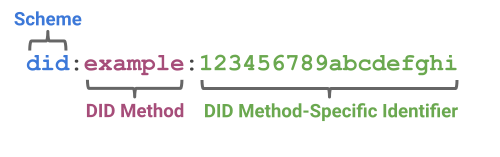
\includegraphics[width=13cm,keepaspectratio]{did-schema.png}
    \centering
    \caption{Composizione di un \gls{did} \cite{img:did-schema}}
    \label{lab:did-schema}
\end{figure}

Un \gls{did} è una stringa composta da tre parti (\autoref{lab:did-schema}): lo schema did:, un metodo e un identificatore univoco rispetto al metodo \cite{wiki:did}. \\
I documenti \gls{did}, invece, sono dei file JSON-LD \cite{wiki:json-ld}. Il documento \gls{did} contiene tutte le informazioni, o claims,
relative al soggetto identificato dal \gls{did} e fornisce una serie di meccanismi che consentono a un controller del \gls{did} di dimostrare il proprio controllo sul \gls{did}.
Tipicamente esprimono anche metodi di verifica, come chiavi pubbliche crittografiche, e servizi relativi alle interazioni con il soggetto \gls{did}. \\
Il controller di un \gls{did} è l'entità che ha la capacità di apportare modifiche a un documento \gls{did}. Questa capacità in genere è subordinata dal possesso dal possesso della coppia di chiavi crittografiche.
Si noti che un \gls{did} potrebbe avere più di un controller e il soggetto \gls{did} può essere il controller \gls{did} o uno di essi. \\
I sistemi che supportano la registrazione dei \gls{did} e la restituzione dei dati necessari per produrre documenti \gls{did} sono chiamati "verifiable data registry". \\
Un risolutore \gls{did} è il componente che, dato un \gls{did}, restituisce il documento corrispondente. Questo processo è chiamato risoluzione \gls{did} (\autoref{lab:did-architecture}).

\begin{figure}[ht]
    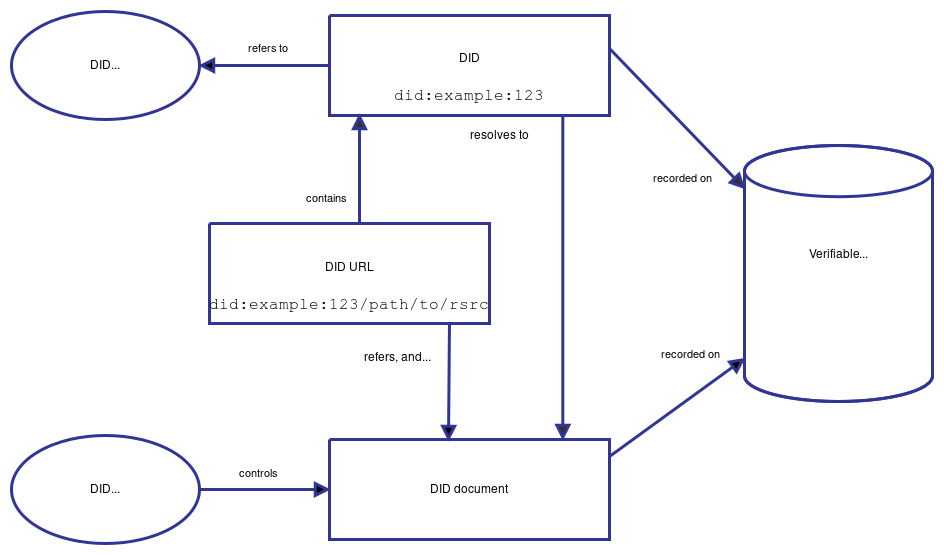
\includegraphics[width=13cm,keepaspectratio]{did-architecture.png}
    \centering
    \caption{Panoramica dell'architettura dei \gls{did} e le relazioni fra le componenti fondamentali \cite{img:did-architecture}}
    \label{lab:did-architecture}
\end{figure}

Il soggetto identificato ha bisogno di un’identità per essere in grado di dimostrare di possedere determinati tratti o caratteristiche a un verificatore. \\
Il verificatore ha un certo numero di emittenti di fiducia ed è disposto ad accettarne i claims, cioè le affermazioni.
Il soggetto può chiedere a uno di questi emittenti di aggiungere una dichiarazione firmata sul proprio documento \gls{did}.
Inoltre, sia l'emittente che il verificatore devono essere in grado di verificare che il soggetto sia effettivamente il proprietario dell'identità.
Ciò si ottiene tramite DIDAuth. \\
Questo processo può assumere molte forme, come specificato nel documento \gls{did}, ma un modo comune è attraverso un challenge inviata dall'emittente o dal verificatore al soggetto,
del quale conoscono la chiave pubblica grazie al DID document, che a sua volta risponderà firmando con la propria chiave privata, dimostrando la propria identità.

\subsubsection {Analogia con il mondo reale}
Si vuole comprare alcool al bar. Per farlo, si deve essere in grado di dimostrare al barista di avere almeno 18 anni. Il barista in questo caso è il verificatore.
Si può dimostrare la richiesta mostrando la propria carta d'identità.
Questa viene rilasciato dal governo, che funge da emittente di fiducia per il barman,
il quale verificherà che il richiedente sia effettivamente la persona raffigurata nella foto e si convincerà che del possesso del requisito della maggiore età.

\begin{figure}[ht]
    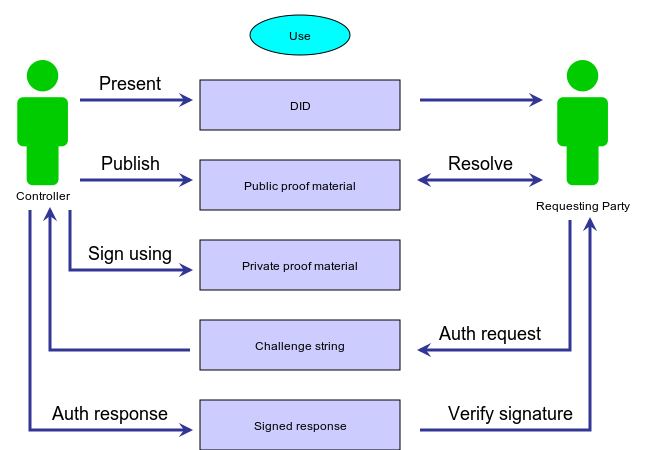
\includegraphics[width=13cm,keepaspectratio]{did-auth.png}
    \centering
    \caption{Panoramica dell'architettura dei \gls{did} e le relazioni fra le componenti fondamentali \cite{img:did-auth}}
    \label{lab:did-auth}
\end{figure}

Le blockchain, grazie alle loro caratteristiche, si sono rivelate un sistema ideale per integrare un sistema di \gls{ssi}, anche in ambiti che esulano il settore energetico \cite{art:blockchain-did}. \\
Nel progetto di \gls{ew} i \gls{did} ricoprono un ruolo centrale.
Ogni utente può richiedere un \gls{did} che mantenga la lista di claims verificabili che l'utente possiede.
È anche possibile assegnare un \gls{did} ad ogni \gls{der}, così da tenere traccia di tutte le informazioni e certificazioni legate a quello specifico \gls{der}. \\

Altri vantaggi forniti da questo sistema sono:
\begin{itemize}
    \item Meccanismo di autenticazione - Il soggetto è in grado di fornire una prova crittografica del proprio controllo sul \gls{did}
    \item Autorizzazione e deleghe -  Il protocollo prevede la possibilità per un \gls{did} di autorizzare o delegare un altro \gls{did} per permettergli di effettuare operazioni a suo nome
\end{itemize}

\section{Identity and Access Management (IAM)}
\label{sec:iam}

\gls{iam} è un insieme di policy in grado di garantire che solo le entità con le credenziali e le autorizzazioni necessarie possano accedere alle risorse. \\
Il sistema deve prima controllare l'identità digitale del soggetto e verificare i ruoli ad esso associati.
L'operazione viene autorizzata solo se il soggetto ha i ruoli necessari.
Per assicurare l'\textit{accountability}, viene utilizzato un sistema di \textit{logging} per registrare ogni operazione eseguita dal soggetto.\\

Per implementare un sistema IAM decentralizzato bisogna garantire alcune proprietà.

\textbf{L'IAM deve essere resistente alla censura.}
Significa che non esiste alcun attore nel sistema che abbia il potere di limitare selettivamente le informazioni a cui gli altri hanno accesso.
Questo aspetto è importante perché informazioni riguardanti situazioni casi in cui un'autorizzazione o una chiave è stata revocata o invalidata o se è stata appena concessa un'autorizzazione devono essere disponibili pubblicamente. \\
Una blockchain, per sua natura, soddisfa questi requisiti. Inoltre, le prove crittografiche contenute nelle transazioni consentono la verifica off-line dei dati.
Le descrizioni dei ruoli sono contenute in uno smart contract ENS, mentre l'avvenuta concessione di un ruolo e i suoi dettagli è annotata nel documento DID dell'utente, mantenuto off-chain.

\textbf{Le informazioni su utenti e ruoli devono essere riservate.}
Nella soluzione di Energy Web, nessuna terza parte dispone dell'elenco completo degli utenti di un'applicazione. \\
Ciò è garantito dal processo di concessione dell'autorizzazione, poiché è l'utente che archivia il claim e ne aggiunge la descrizione sulla blockchain, consentendogli di dimostrare che gli è stato concessa una determinata autorizzazione (\autoref{lab:iam-process}). \\
Poiché si tratta di una operazione svolta dall'utente stesso, i contenuti del ruolo non sono divulgati \cite{img:iam}.
L'unica informazione che un osservatore può raccogliere è che l'utente ha aggiunto un claim al proprio DID document, ma non il contenuto, l'origine o la natura del claim. \\

\begin{figure}[ht]
    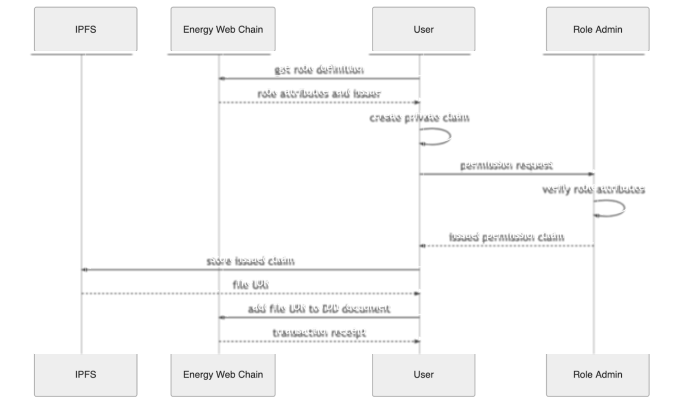
\includegraphics[width=13cm,keepaspectratio]{iam-process.png}
    \centering
    \caption{Processo di rilascio dei ruoli \gls{iam} \cite{img:iam}}
    \label{lab:iam-process}
\end{figure}

Anche l'\gls{iam} rappresenta un punto cardine nel progetto \gls{ew}. \\
Attraverso il suo utilizzo, è possibile creare delle organizzazioni con una struttura gerarchica, simile ai domini attualmente utilizzati sul web.
I ruoli che gli utenti possiedono determinano le azioni che possono compiere all'interno dell'organizzazione. \\
La gestione di tutti questi aspetti è stata resa molto più accessibile grazie alla \gls{dapp} \href{https://switchboard.energyweb.org/}{Switchboard} (\url{https://switchboard.energyweb.org/}).